% ************************** Prólogo *****************************
% Use `prologo' as an option in the document class to print only the titlepage and the abstract.

\begin{prologo}

\subsection*{Presentación}
El presente Trabajo Fin de Máster en Tecnologías de la Información Geográfica para la Ordenación del Territorio: SIG y Teledetección, expone todas las tareas que se han realizado durante la colaboración en el Proyecto SIOSE-INNOVA: Innovaciones técnicas y metodológicas en el Sistema de Información sobre Ocupación del Suelo de España (SIOSE) y su aplicación en estudios geográficos. El investigador principal de este proyecto es Alfredo Ramón Morte, que cuenta con la participación de los miembros del Laboratorio de Geomática y otros profesionales, en colaboración con el equipo de investigación responsable de la base de datos del SIOSE.

Todo este trabajo se ha realizado mediante el marco de convenio de prácticas de empresa entre la Universidad de Zaragoza y el Laboratorio de Geomática del Instituto Interuniversitario de Geografía de la Universidad de Alicante. El periodo de prácticas ha tenido una duración desde julio hasta noviembre de 2017, de un total de 440 horas (ver en el \nameref{chap:anexoIV}).

El Laboratorio de Geomática se encarga de administrar el Sistema de Información Geográfica de la Universidad de Alicante (SIGUA), o como era conocido al principio, Laboratorio de SIG y Cartografía Automatizada. Este cambio de nombre fue razón por la orientación del laboratorio al desarrollo de soluciones basadas en la geomática o informática aplicada a la Geografía.

Su origen data de 1997, año en el que además, se pone en marcha el servicio SIGUA, que gran parte de los empleados se centran en el mantenimiento del sistema, como también de la creación de nuevas utilidades adaptadas a las necesidades de la Universidad de Alicante y, compartir recursos e interconectar sistemas de información por otras unidades. Cabe mencionar que, está formado por licenciados en Geografía y en Informática que desarrollan su trabajo en las Tecnologías de la Información Geográfica basado en software libre.

\subsection*{Proyecto SIOSE-INNOVA}
SIOSE-INNOVA es un proyecto de investigación financiado por el Programa Estatal de Investigación, Desarrollo e Innovación Orientada a los Retos de la Sociedad, dentro del marco Plan Estatal de Investigación Científica y Técnica y de Innovación 2013-2016. Los objetivos principales tienen una parte innovadora, que consiste en comprobar qué tecnologías NoSQL (no sólo SQL) pueden aportar mejores soluciones para la explotación de la base de datos del SIOSE, y una parte aplicada, que consiste en poner en práctica las nuevas tecnologías en casos de estudios reales.

Durante el desarrollo del proyecto, se quieren alcanzar los siguientes objetivos específicos:
\begin{enumerate}
\item Crear un marco de experimentación reproducible y fácilmente utilizable por un gran número de usuarios.
\item Analizar las necesidades y rendimiento de distintas tecnologías de bases de datos NoSQL para la explotación del SIOSE.
\item Desarrollar e implementar un nuevo modelo de datos auxiliar que permita extender las posibilidades de análisis del SIOSE con técnicas de Big Data o Data Mining.
\item Evaluar la usabilidad de los datos SIOSE en distintas plataformas tecnológicas, mediante su aplicación en casos de uso reales en los que utilizar datos de ocupación del suelo resulte esencial.
\end{enumerate}

A partir de estos objetivos, el proyecto SIOSE-INNOVA tiene como objetivo final crear un visor cartográfico donde se pueda consultar y comparar resultados entre distintos paisajes (ver figura \ref{fig:visorweb}). Por este motivo, se desarrolla una nueva extensión denominada \textit{pg\_landmetrics} capaz de calcular métricas del paisaje, papel fundamental para este trabajo.

\begin{figure}
\begin{center}
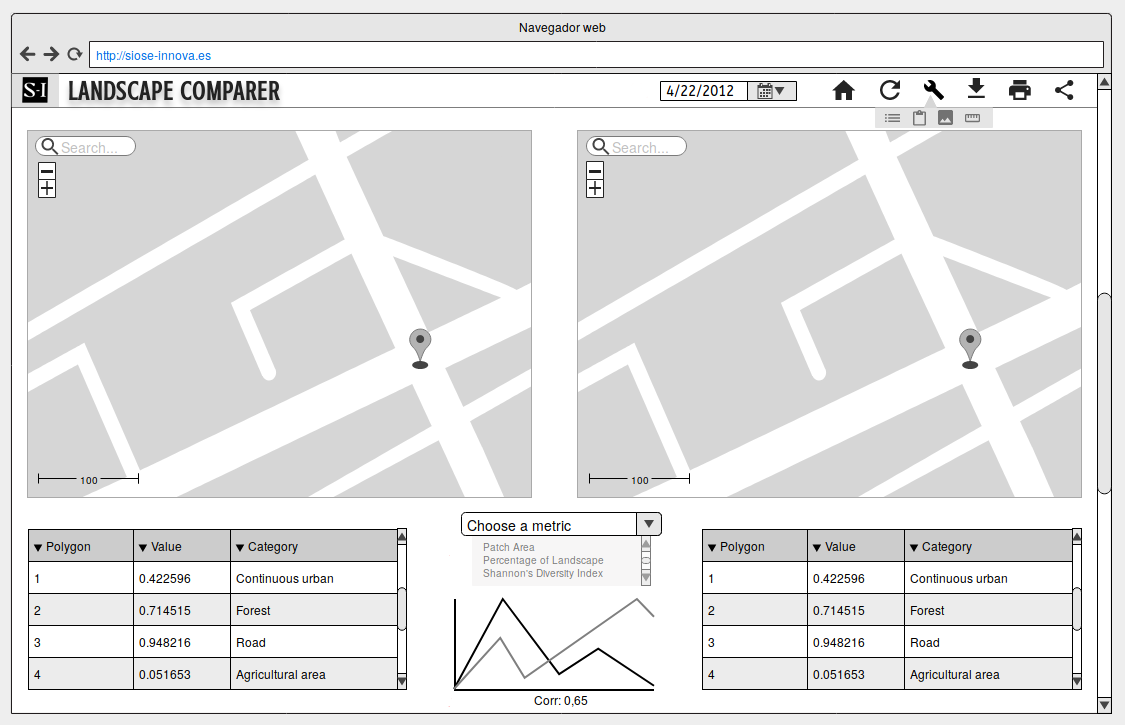
\includegraphics[width=\textwidth]{Prologo/Figs/visorweb.png}
\caption{Prototipo del visor cartográfico. \label{fig:visorweb}}
\end{center}
\end{figure}

Las métricas de paisaje son importantes para el estudio del paisaje en su estructura, comportamiento o modificación temporal, ya sea por factores naturales como artificiales. Es por este motivo la necesidad de crear una extensión que permita aplicarlas y calcularlas sobre el paisaje.\\

\subsection*{Estructura del trabajo}
Este trabajo se organiza en cuatro capítulos, a parte las referencias bibliográficas y los anexos, y su estructura es la siguiente:
\begin{itemize}
\item En el capítulo \ref{chap:intro} se analiza la estructura del paisaje a partir del uso y cobertura del suelo en relación con las métricas de paisaje. Además, se desarrollan los objetivos que se quieren alcanzar en el trabajo.

\item En el capítulo \ref{chap:metod} se describen todos los procesos necesarios para implementar y desarrollar la nueva extensión PostgreSQL/PostGIS, desde el conjunto de datos hasta las tareas diarias, la incorporación de funciones y la documentación de la extensión.

\item En el capítulo \ref{chap:result} se detallan todos los resultados que se obtienen a partir de la extensión en casos reales.

\item Por último, en el capítulo \ref{chap:concl} se realiza un análisis conclusivo para  Además, se describen las aportaciones interesantes para trabajos futuros.
\end{itemize}



\end{prologo}
